
\textit{Braille music compiler} est un programme qui a pour objectif
de transformer un fichier écrit en \textit{Braille Music} en un autre
langage utilisable par d'autres applications. La difficulté est que le
langage \textit{Braille Music} possède beaucoup d'ambiguïtés, en effet
par exemple pour connaître la note exacte en cours, il est nécessaire
de savoir quelles ont été les notes précédentes. \`A l'heure actuelle
le programme arrive correctement à compiler le langage \textit{Braille
  Music} en un langage Abstrait qui lui ne possède aucune
ambiguïté. Ce langage abstrait peut être converti en n'importe quels
formats de musique. Par exemple :

\begin{itemize}
\item MIDI (Format AUDIO)
\item MusicXML 
\item lilypond (Equivalent au Latex, mais pour la musique)
\end{itemize}
Le schéma \ref{compiler} résume le fonctionement de BMC.

\begin{figure}[!h]
  \centering
  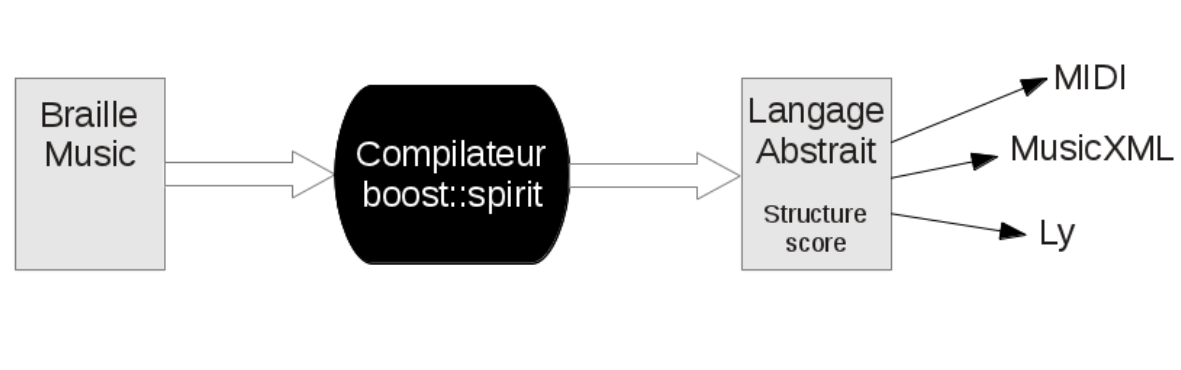
\includegraphics[width=1\textwidth]{images/fonction-bmc.png}
  \caption{Schéma visuel du fonctionement de BMC}
  \label{compiler}
\end{figure}

Notre travail a été d'implémenter quelque uns de ces modules de
conversion. Pour cela il est nécessaire de comprendre comment est
conçu le langage Abstrait. Après la compilation du \textit{Braille
  Music}, l'ensemble des données sont stockées dans une structure
nommée "score". Cette structure est une multitude de vecteurs
imbriqués les uns dans les autres. Voici le code de la strucure suivi
d'une représentation visuel (\ref{score}) :

\begin{verbatim}
typedef boost::variant<note, rest, chord, value_distinction, hand_sign, simile, barline>;
typedef std::vector<sign> partial_voice;
typedef std::vector<partial_voice> partial_measure;
typedef std::vector<partial_measure> voice;
struct measure : locatable
{
  boost::optional<unsigned> ending;
  std::vector<voice> voices;
};
typedef std::vector< boost::variant<measure> > staff;
typedef std::vector<staff> part;
struct score {
  boost::optional<time_signature> time_sig;
  std::vector<part> parts;
};
\end{verbatim}

\begin{figure}[h]
  \centering
  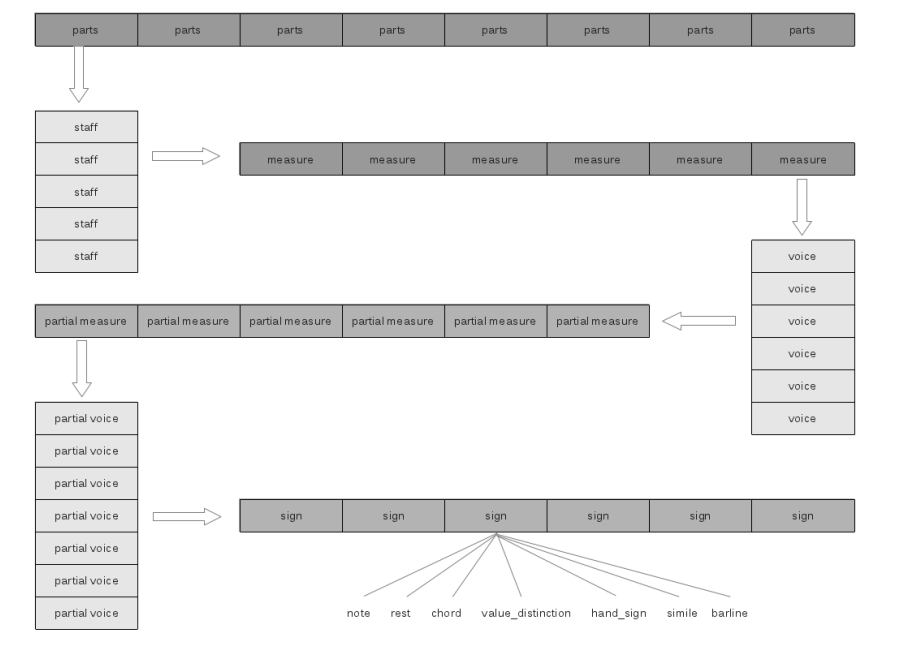
\includegraphics[width=1\textwidth]{images/bmc-score.png}
  \caption{Représentation de la structure score}
  \label{score}
\end{figure}

Il est donc maintenant plus facile d'expliquer la structure
\textit{score}. Un fichier de musique braille peut donc se diviser en
plusieurs parties (parts). Chaque partie possède un ou plusieurs
"staff". Un "staff" n'est autre que la portée, typiquement si le
compositeur écrit une partition de musique pour piano il y aura deux
portées. Chaque portée possède un nombre de mesures. Si la musique
composée est polyphonique il y aura plusieurs voix ("voices"). Une
voix est ensuite divisée en mesures partielles, ces mesures partielles
pouvant de nouveau être divisées en voix ("partial\_voices") qui elles
sont divisées en un vecteur de \textit{sign}. Un sign pouvant être une
note, un repos, une barre ... La figure \ref{musicexe} représente sur
une partition de musique ses différents termes.


\begin{figure}[!h]
  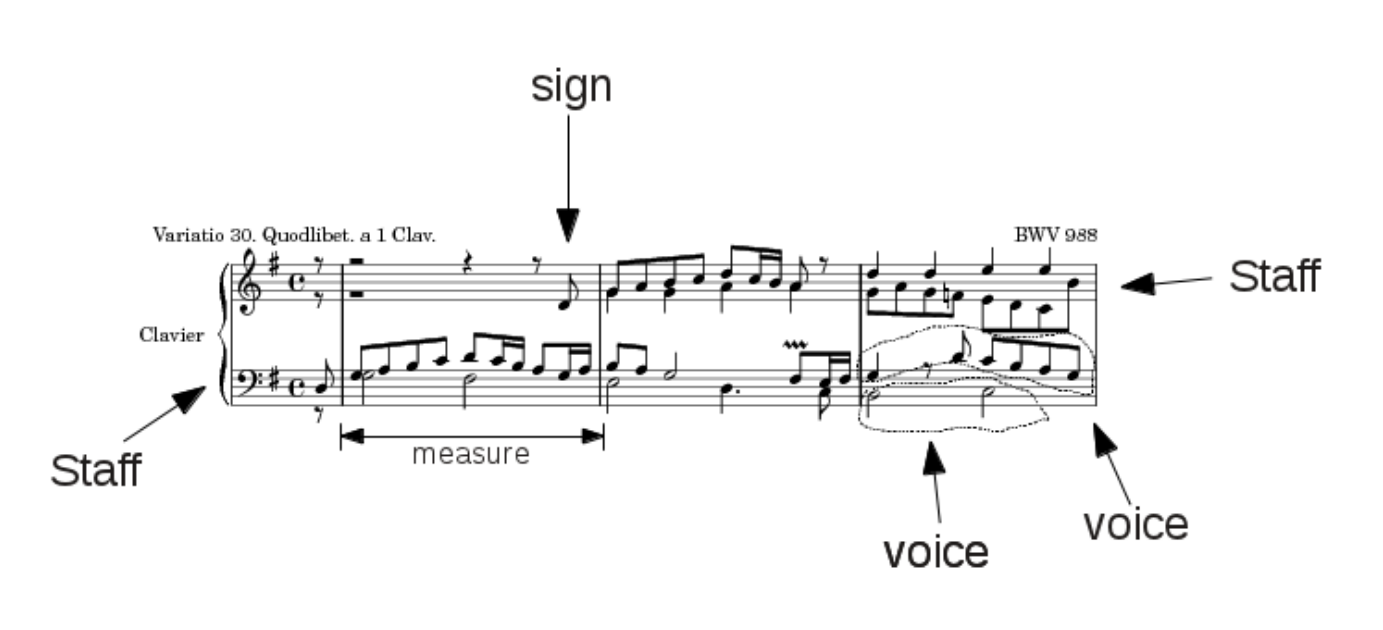
\includegraphics[width=1\textwidth]{images/score-visu.png}
  \caption{Un petit exemple visuel}
  \label{musicexe}
\end{figure}

À partir de ce langage intermédiaire nous avons pu réaliser deux
classes qui ont été intégré dans le programme bmc. Chaqu'une d'elle
créer un fichier représentant une partition braille passée en argument
dans un autre langage.


